\documentclass[11pt,a4paper]{article}

\usepackage[T1]{fontenc}
\usepackage[utf8]{inputenc}
\usepackage{mathpazo}
\usepackage[scaled=0.92]{helvet}
\renewcommand{\ttdefault}{lmtt}
\usepackage[margin=2.4cm]{geometry}
\usepackage{amsmath}
\usepackage{graphicx}
\usepackage{booktabs}
\usepackage{array}
\usepackage{enumitem}
\usepackage{tikz}
\usetikzlibrary{arrows.meta,positioning,calc}
\usepackage{xcolor}
\usepackage{titlesec}
\usepackage{fancyhdr}
\usepackage[colorlinks=true,linkcolor=black,urlcolor=blue!50!black]{hyperref}

\graphicspath{{figures/}}
\setlength{\parindent}{0pt}
\setlength{\parskip}{0.55em}
\setlist{itemsep=0.15em,topsep=0.2em}
\renewcommand{\arraystretch}{1.25}

\titleformat{\section}{\Large\bfseries\sffamily}{\thesection}{0.6em}{}
\titleformat{\subsection}{\large\bfseries\sffamily}{\thesubsection}{0.6em}{}
\titlespacing*{\section}{0pt}{1.6em}{0.5em}
\titlespacing*{\subsection}{0pt}{1.1em}{0.3em}

\pagestyle{fancy}
\fancyhf{}
\fancyhead[L]{\small\sffamily Lung segmentation hands-on: the theory you need}
\fancyhead[R]{\small\sffamily\thepage}
\renewcommand{\headrulewidth}{0.3pt}

% "Where it is used" line under a section title
\newcommand{\usedin}[1]{{\small\sffamily\color{black!60}Used in: #1}\par\vspace{0.2em}}
% Key term
\newcommand{\term}[1]{\textbf{#1}}
% Code
\newcommand{\code}[1]{\texttt{\small #1}}
% A short framed summary at the end of a section
\newcommand{\remember}[1]{%
  \par\vspace{0.4em}\noindent\fcolorbox{black!35}{black!4}{\parbox{\dimexpr\linewidth-2\fboxsep-2\fboxrule}{%
  \textbf{\sffamily Remember.} #1}}\par}

\begin{document}

\begin{center}
{\LARGE\bfseries\sffamily Lung segmentation hands-on}\\[0.4em]
{\Large\sffamily The theory you need}\\[0.8em]
{\small MSc Health Informatics, Advanced Topics in Machine Learning}
\end{center}

\vspace{0.5em}

This handbook contains the ideas behind the exercises, and nothing else. It follows the order of the course:
each section says in which notebook it is used. Read a section before the corresponding part, and come back to
it when a step of the project is not clear. The last page is an index of the terms.

\vspace{0.3em}
\begin{center}
\begin{tabular}{@{}cll@{}}
\toprule
Section & Topic & Used in \\
\midrule
1 & CT images & Notebook 01 \\
2 & Files: DICOM and NIfTI & Notebook 01 \\
3 & Preparing the data for a network & Notebook 02; project STEP 3--5 \\
4 & The segmentation network & Project STEP 6 \\
5 & Loss and metric: the Dice & Project STEP 7 \\
6 & Training & Project STEP 8--11 \\
7 & Is the model good? & Project STEP 12 \\
8 & Using the model & Project STEP 13; web app \\
9 & Lung nodules and experiments & Notebook 04 \\
10 & From a model to a web app & Day 5 \\
\bottomrule
\end{tabular}
\end{center}

% ---------------------------------------------------------------------------
\section{CT images}
\usedin{notebook 01, sections 2--6}

\subsection{An image is a matrix of numbers}

A CT scanner sends X-rays through the body from many angles and computes how much each small piece of the
body attenuates them. The result is a stack of \term{slices}. One slice is a matrix, usually of
$512 \times 512$ numbers: each number is one \term{pixel}. Stacking the slices gives a 3D array; an element of
it is called a \term{voxel}.

In Python a slice is a NumPy array. Everything we do, from plotting to training, is arithmetic on arrays.

\subsection{Hounsfield units}

The numbers of a CT image have a physical meaning. They are expressed in \term{Hounsfield units (HU)}, a scale
where water is 0 and air is $-1000$. Dense tissue attenuates more and has higher values.
The scale is the same on every scanner, which is why a model trained on scans from one hospital can read
scans from another.

\begin{center}
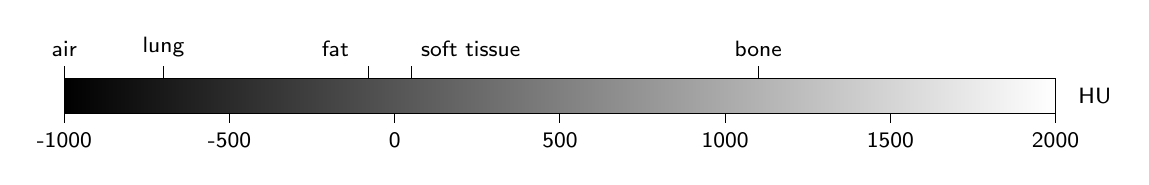
\begin{tikzpicture}[font=\footnotesize\sffamily, x=0.0042cm]
\shade[left color=black, right color=white] (-1000,0) rectangle (2000,0.45);
\draw (-1000,0) rectangle (2000,0.45);
\foreach \x in {-1000,-500,0,500,1000,1500,2000} { \draw (\x,0) -- (\x,-0.12) node[below] {\x}; }
\foreach \x/\t in {-1000/air, -700/lung, -80/fat, 50/soft tissue, 1100/bone} { \draw (\x,0.45) -- (\x,0.6); }
\node[above] at (-1000,0.6) {air};
\node[above] at (-700,0.6) {lung};
\node[above] at (-180,0.6) {fat};
\node[above] at (230,0.6) {soft tissue};
\node[above] at (1100,0.6) {bone};
\node[right] at (2040,0.22) {HU};
\end{tikzpicture}
\end{center}

\begin{center}
\begin{tabular}{@{}lr@{}}
\toprule
Tissue & HU (approximate) \\
\midrule
Air & $-1000$ \\
Lung & $-900$ to $-500$ \\
Fat & $-100$ to $-50$ \\
Water & $0$ \\
Soft tissue (muscle, organs, blood) & $20$ to $80$ \\
Bone & $300$ to $2000$ \\
\bottomrule
\end{tabular}
\qquad
\raisebox{-0.5\height}{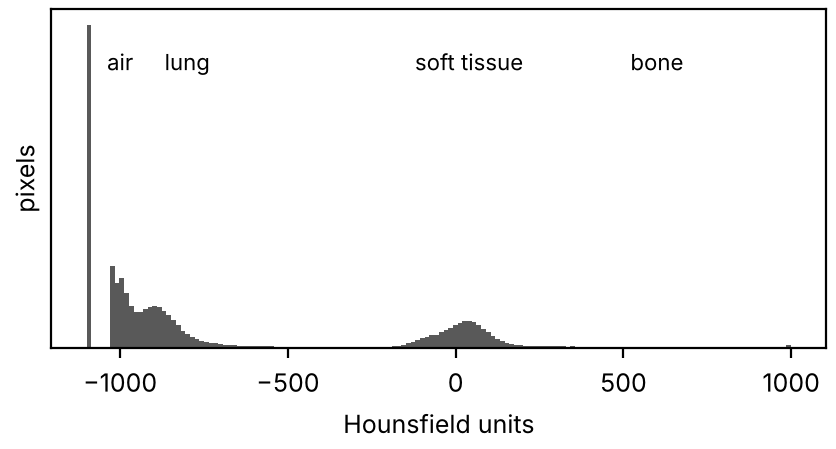
\includegraphics[width=0.48\linewidth]{histogram.png}}
\end{center}

Lung is mostly air, so it is much darker than everything around it. This contrast is what makes lung
segmentation an easy task.

Some scans contain values far below $-1000$ (for example $-2000$ or $-3024$) outside the circular area
measured by the scanner. They are not tissue and must be cut away.

\subsection{Windowing}

A CT image has thousands of different values, a screen shows a few hundred grey levels. A \term{window} is a
range of HU, from $\mathrm{HU}_{\min}$ to $\mathrm{HU}_{\max}$, that is stretched over the whole grey scale.
Values below the range become black, values above become white.

\begin{center}
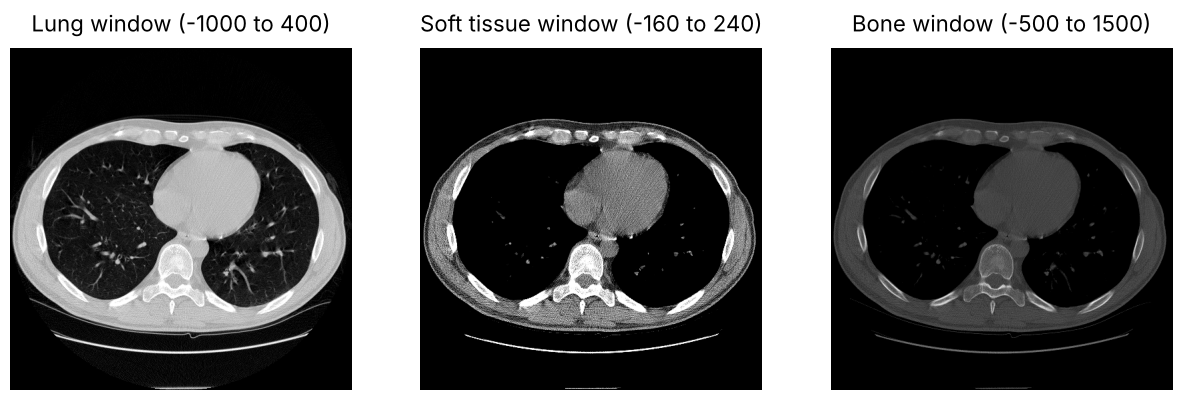
\includegraphics[width=0.95\linewidth]{windows.png}
\end{center}

The same operation prepares the image for a neural network, which works best with small numbers. We cut the
values to the window and rescale them between 0 and 1:
\[
x_{\text{scaled}} = \frac{\operatorname{clip}(x,\ \mathrm{HU}_{\min},\ \mathrm{HU}_{\max}) - \mathrm{HU}_{\min}}
{\mathrm{HU}_{\max} - \mathrm{HU}_{\min}}
\]
In the course we always use $\mathrm{HU}_{\min} = -1000$ and $\mathrm{HU}_{\max} = 400$.

\subsection{Segmentation masks}

To \term{segment} an image means to decide, for every pixel, which structure it belongs to. The answer is a
\term{mask}: an image of the same size where each pixel holds a \term{label}, a whole number. In the project:
0 for background, 1 for lung.

\begin{center}
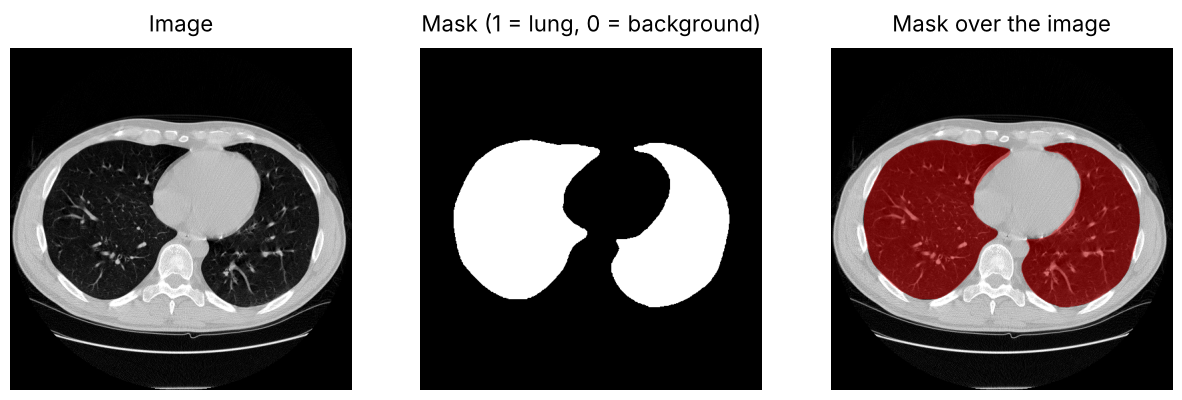
\includegraphics[width=0.95\linewidth]{mask.png}
\end{center}

The masks we use as the correct answer are called \term{ground truth} or reference. In our dataset they were
produced by an automatic program, not drawn by radiologists: most are very good, a few are wrong.

\subsection{Pixel spacing}

A pixel covers a small area of the patient. Its side, in millimetres, is the \term{pixel spacing}; the distance
between two slices is the \term{slice thickness}. Both are written in the file and change from scan to scan.
They turn counts of pixels into real measurements:
\[
\text{area (cm}^2) = \frac{\text{number of pixels} \times \text{spacing}_x \times \text{spacing}_y}{100}
\]

\remember{A CT slice is a matrix of Hounsfield units. A window selects the range we care about. A mask gives
one label per pixel. The spacing converts pixels to millimetres.}

% ---------------------------------------------------------------------------
\section{Files: DICOM and NIfTI}
\usedin{notebook 01, sections 7--9}

A medical image file contains the pixels and a \term{header}: information on how to interpret them (size,
spacing, position in the patient).

\begin{center}
\begin{tabular}{@{}p{3.2cm}p{5.6cm}p{5.6cm}@{}}
\toprule
 & DICOM (\code{.dcm}) & NIfTI (\code{.nii}, \code{.nii.gz}) \\
\midrule
Where it is used & hospitals, scanners & research, deep learning \\
One scan is & a folder with one file per slice & one file \\
Pixel values & raw integers, to be converted & ready to use \\
Patient data & name, date of birth, \dots & none \\
Python library & \code{pydicom} & \code{nibabel} \\
\bottomrule
\end{tabular}
\end{center}

\begin{center}
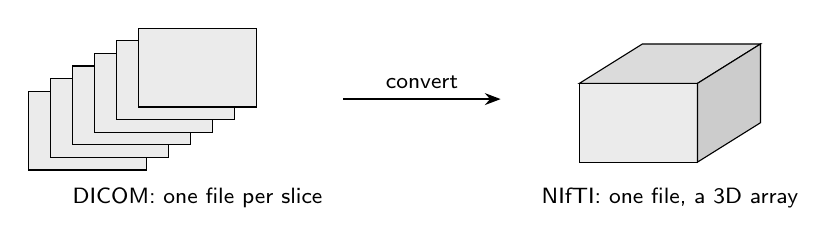
\begin{tikzpicture}[font=\footnotesize\sffamily]
\foreach \i in {0,...,5} { \draw[fill=black!8] (\i*0.28,\i*0.16) rectangle ++(1.5,1.0); }
\node at (2.15,-0.35) {DICOM: one file per slice};
\draw[-{Stealth[length=2mm]}, thick] (4.0,0.9) -- node[above] {convert} (6.0,0.9);
\draw[fill=black!8] (7.0,0.1) -- ++(1.5,0) -- ++(0,1.0) -- ++(-1.5,0) -- cycle;
\draw[fill=black!14] (7.0,1.1) -- ++(0.8,0.5) -- ++(1.5,0) -- ++(-0.8,-0.5) -- cycle;
\draw[fill=black!20] (8.5,0.1) -- ++(0.8,0.5) -- ++(0,1.0) -- ++(-0.8,-0.5) -- cycle;
\node at (8.15,-0.35) {NIfTI: one file, a 3D array};
\end{tikzpicture}
\end{center}

\textbf{DICOM values.} A DICOM file stores raw integers. Two numbers in the header convert them to Hounsfield
units:
\[
\mathrm{HU} = \text{stored value} \times \text{RescaleSlope} + \text{RescaleIntercept}
\]

\textbf{Order of the slices.} The files of a DICOM folder are not guaranteed to be in order. The position of
each slice along the body is the third number of the tag \code{ImagePositionPatient}: sort by it before
stacking the slices.

\textbf{Privacy.} DICOM headers contain personal data. Files must be anonymised before they leave the hospital.

\textbf{Orientation.} By convention an axial slice is shown as if we looked at the patient from the feet: the
patient's right side is on the left of the picture. In our files the first axis of the array is $x$, so we plot
the transposed array, \code{image.T}.

\remember{DICOM is the clinical format: many files, raw values, personal data. NIfTI is the research format:
one file, values in HU, no personal data. We work with NIfTI.}

% ---------------------------------------------------------------------------
\section{Preparing the data for a network}
\usedin{notebook 02; project STEP 3, 4 and 5}

\subsection{Tensors and shapes}

PyTorch works with \term{tensors}: arrays that can live on the \term{GPU}, a processor that does the
same simple operation on millions of numbers at once. Training a network on a GPU takes minutes; on a normal
processor, hours. The network expects a precise
\term{shape}. For a group of 2D images it is
\[
(\text{batch},\ \text{channels},\ \text{height},\ \text{width}) \qquad\text{for example}\qquad (16,\ 1,\ 256,\ 256)
\]
\begin{center}
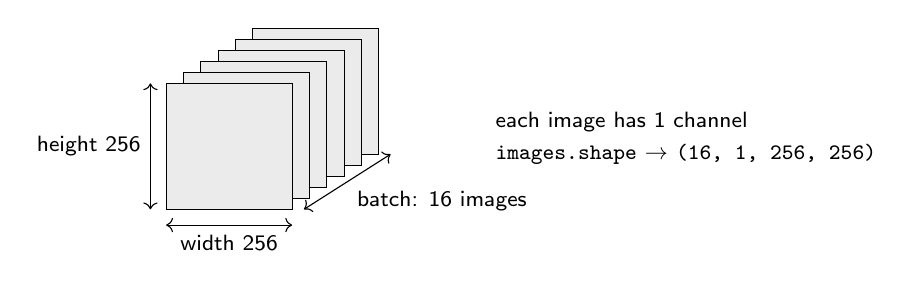
\begin{tikzpicture}[font=\footnotesize\sffamily]
\foreach \i in {5,4,...,0} { \draw[fill=black!8] (\i*0.22,\i*0.14) rectangle ++(1.6,1.6); }
\draw[<->] (0,-0.2) -- node[below] {width 256} (1.6,-0.2);
\draw[<->] (-0.2,0) -- node[left] {height 256} (-0.2,1.6);
\draw[<->] (1.75,0.0) -- node[below right] {batch: 16 images} (2.85,0.7);
\node[align=left] at (6.6,0.9) {each image has 1 channel\\[2pt]\texttt{images.shape} $\rightarrow$ \texttt{(16, 1, 256, 256)}};
\end{tikzpicture}
\end{center}

\begin{itemize}
\item \term{Batch}: how many images are processed together (16). A larger batch is faster but needs more
memory; if the GPU runs out of memory, reduce the batch size.
\item \term{Channels}: how many values each pixel has. A CT slice has 1; a colour photo has 3.
\item Height and width: all the images of a batch must have the same size.
\end{itemize}
When something fails in PyTorch, the first thing to do is to print the shapes.

\subsection{Transforms}

A \term{transform} is a function that does one step of the preparation. The steps of our pipeline:

\begin{center}
\begin{tabular}{@{}clp{8.3cm}@{}}
\toprule
 & MONAI transform & What it does \\
\midrule
1 & \code{LoadImaged} & reads the files \\
2 & \code{EnsureChannelFirstd} & adds the channel: $(512, 512) \rightarrow (1, 512, 512)$ \\
3 & \code{Lambdad} with our function & label: lung $\rightarrow 1$, everything else $\rightarrow 0$ \\
4 & \code{ScaleIntensityRanged} & image: window $-1000/400$ HU rescaled to $0/1$ (section 1.3) \\
5 & \code{Resized} & image and label to $256 \times 256$ \\
\bottomrule
\end{tabular}
\end{center}

\code{Compose} chains them. The final \code{d} in the names means that the transform works on a
\term{dictionary} \code{\{"image": ..., "label": ...\}}, so image and mask go through the same steps.

\begin{center}
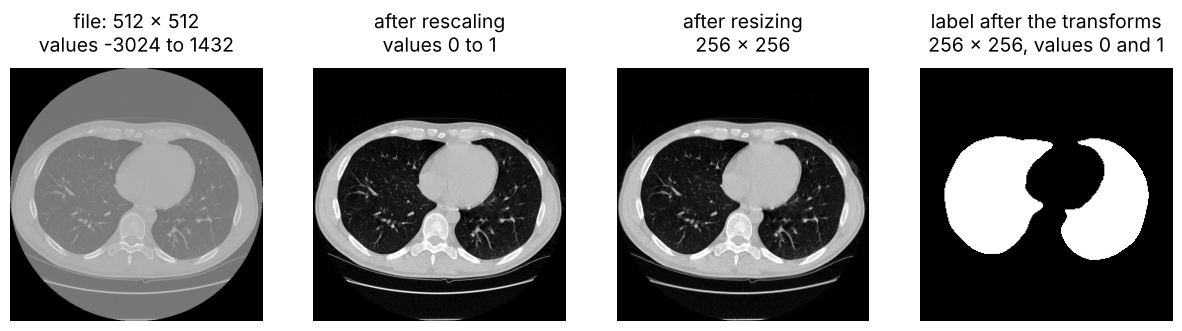
\includegraphics[width=0.98\linewidth]{pipeline.png}
\end{center}

\textbf{Interpolation.} Resizing must invent new pixel values. For the image we use \code{"bilinear"}: each
new pixel is an average of its neighbours. For the mask we use \code{"nearest"}: each new pixel copies the
closest one. An average of the labels 0 and 1 would give 0.5, which is not a label.

\begin{center}
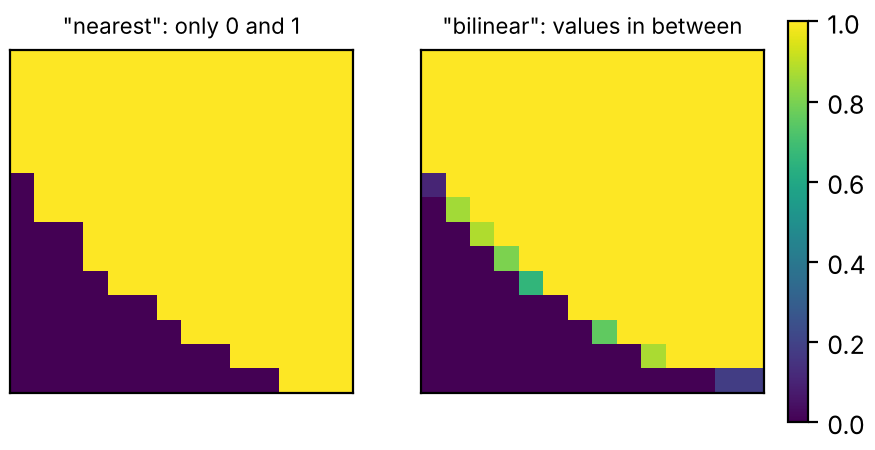
\includegraphics[width=0.62\linewidth]{interpolation.png}

{\small The border of a lung mask after resizing, enlarged.}
\end{center}

\subsection{Data augmentation}

A network learns from examples, and we have few. \term{Data augmentation} shows the network a slightly
different version of each image at every epoch: rotated by a few degrees, a little larger or smaller, shifted.
The network sees more variety and becomes more robust.

\begin{center}
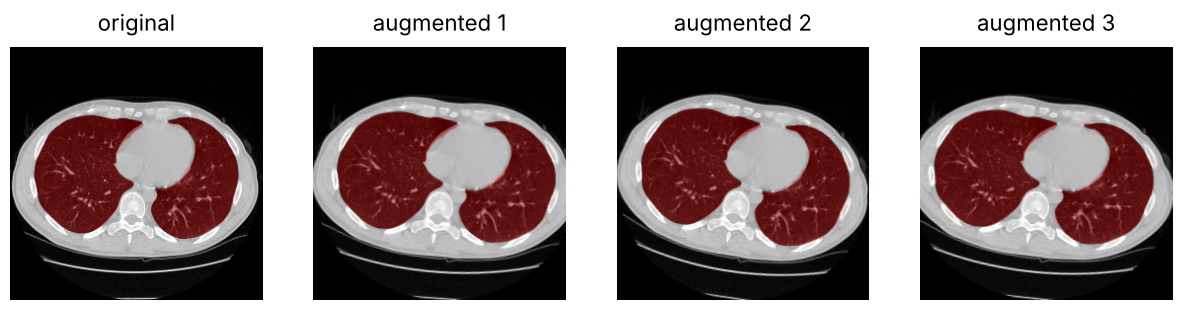
\includegraphics[width=0.95\linewidth]{augmentation.png}
\end{center}

Three rules:
\begin{itemize}
\item the same random change is applied to the image and to its mask;
\item the result must still look like a real image (small changes);
\item augmentation is used \emph{only} on the training set.
\end{itemize}

\subsection{Training, validation and test sets}

We divide the patients in three groups, and each group has one job.

\begin{center}
\begin{tabular}{@{}llp{9cm}@{}}
\toprule
Set & Share & Job \\
\midrule
Training & 70\% & the network learns from these images \\
Validation & 15\% & during the training, tells us how the network does on images it is not learning from; we
use it to choose when to stop \\
Test & 15\% & used once, at the end, to measure the performance we report \\
\bottomrule
\end{tabular}
\end{center}

\begin{center}
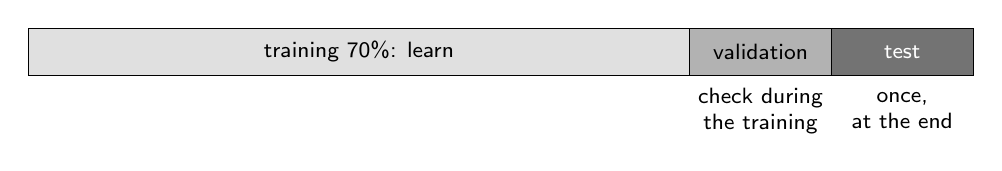
\begin{tikzpicture}[font=\footnotesize\sffamily]
\draw[fill=black!12] (0,0) rectangle (8.4,0.6); \node at (4.2,0.3) {training 70\%: learn};
\draw[fill=black!30] (8.4,0) rectangle (10.2,0.6); \node at (9.3,0.3) {validation};
\draw[fill=black!55] (10.2,0) rectangle (12,0.6); \node[white] at (11.1,0.3) {test};
\node[align=center] at (9.3,-0.45) {check during\\the training};
\node[align=center] at (11.1,-0.45) {once,\\at the end};
\end{tikzpicture}
\end{center}

Why three and not two? Every choice we make by looking at the validation score (how many epochs, which
model to keep) fits the model a little to those patients. Only a set that was never looked at gives an honest
number. All the images of one patient must be in the same set.

\subsection{Dataset and DataLoader}

\begin{itemize}
\item A \term{Dataset} knows how many samples there are and how to produce sample number $i$ (read the files,
apply the transforms).
\item A \term{DataLoader} asks the Dataset for samples and groups them in batches. With \code{shuffle=True}
the order changes at every epoch, which helps the training.
\end{itemize}

\remember{The network wants tensors of shape (batch, channels, height, width) with values between 0 and 1.
Transforms prepare them. Augmentation only for training. The test set is opened once, at the end.}

% ---------------------------------------------------------------------------
\section{The segmentation network}
\usedin{project STEP 6}

\subsection{What a neural network is, in three sentences}

A neural network is a function with millions of adjustable numbers, the \term{weights}. It takes an image and
returns a prediction. \term{Training} means adjusting the weights until the predictions are close to the
correct answers.

\subsection{Convolutions}

The basic operation on images is the \term{convolution}: a small matrix of weights (for example $3 \times 3$),
called a filter, slides over the image and at each position computes a weighted sum of the pixels under it.
One filter detects one local pattern, such as an edge. A \term{layer} applies many filters; the next layer
combines their outputs into more complex patterns.

\begin{center}
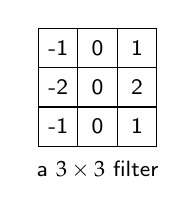
\begin{tikzpicture}[font=\footnotesize\sffamily, baseline=(current bounding box.center)]
\foreach \r/\a/\b/\c in {0/-1/0/1, 1/-2/0/2, 2/-1/0/1} {
  \draw (0,-\r*0.5) rectangle ++(0.5,0.5) node[pos=.5] {\a};
  \draw (0.5,-\r*0.5) rectangle ++(0.5,0.5) node[pos=.5] {\b};
  \draw (1.0,-\r*0.5) rectangle ++(0.5,0.5) node[pos=.5] {\c};
}
\node at (0.75,-1.3) {a $3 \times 3$ filter};
\end{tikzpicture}
\qquad
\raisebox{-0.5\height}{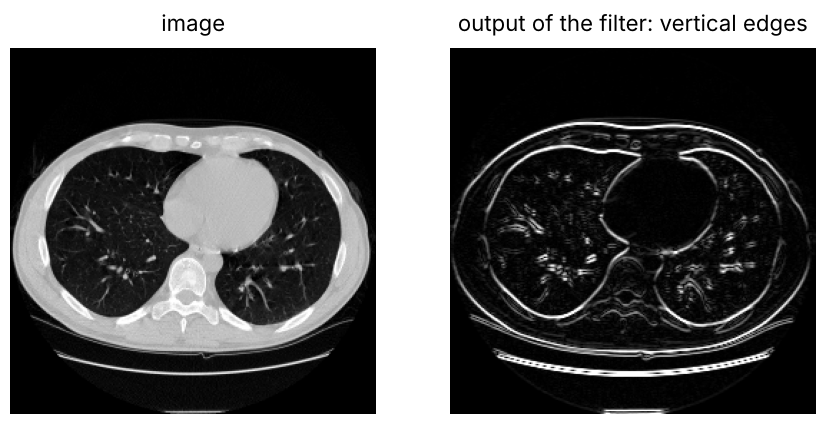
\includegraphics[width=0.6\linewidth]{convolution.png}}

{\small This filter was chosen by hand to find vertical edges. In a network, the numbers of the filters are the
weights: the training chooses them.}
\end{center}

\subsection{The U-Net}

The \term{U-Net} is the standard network for medical image segmentation. It has two halves.

\begin{center}
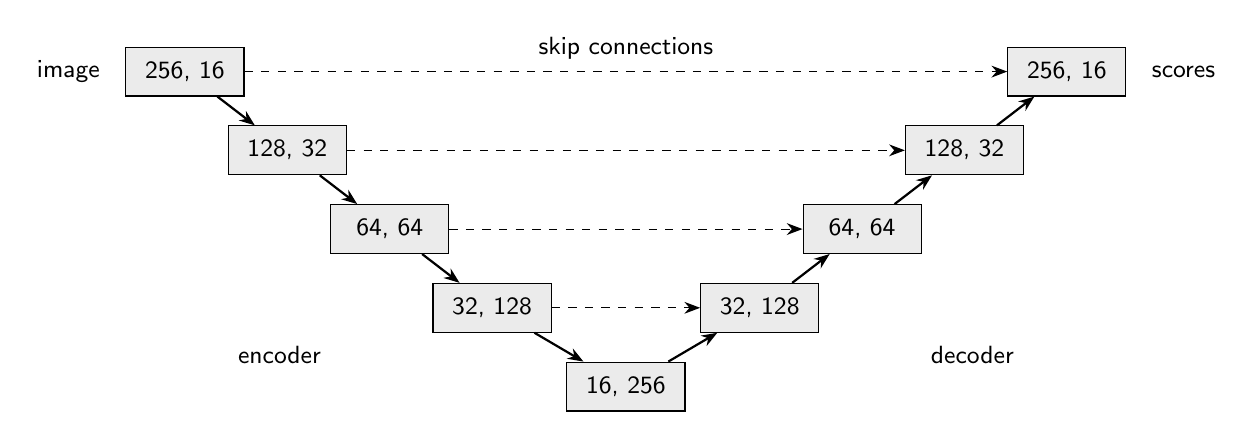
\begin{tikzpicture}[
  blk/.style={draw, fill=black!8, minimum width=1.5cm, minimum height=0.62cm, font=\small\sffamily},
  arr/.style={-{Stealth[length=2mm]}, thick},
  skip/.style={-{Stealth[length=2mm]}, dashed}]
\node[blk] (e1) at (0,0) {256, 16};
\node[blk] (e2) at (1.3,-1) {128, 32};
\node[blk] (e3) at (2.6,-2) {64, 64};
\node[blk] (e4) at (3.9,-3) {32, 128};
\node[blk] (b)  at (5.6,-4) {16, 256};
\node[blk] (d4) at (7.3,-3) {32, 128};
\node[blk] (d3) at (8.6,-2) {64, 64};
\node[blk] (d2) at (9.9,-1) {128, 32};
\node[blk] (d1) at (11.2,0) {256, 16};
\draw[arr] (e1) -- (e2); \draw[arr] (e2) -- (e3); \draw[arr] (e3) -- (e4); \draw[arr] (e4) -- (b);
\draw[arr] (b) -- (d4); \draw[arr] (d4) -- (d3); \draw[arr] (d3) -- (d2); \draw[arr] (d2) -- (d1);
\draw[skip] (e1) -- (d1); \draw[skip] (e2) -- (d2); \draw[skip] (e3) -- (d3); \draw[skip] (e4) -- (d4);
\node[font=\small\sffamily, left=0.2cm of e1] {image};
\node[font=\small\sffamily, right=0.2cm of d1] {scores};
\node[font=\small\sffamily] at (1.2,-3.6) {encoder};
\node[font=\small\sffamily] at (10,-3.6) {decoder};
\node[font=\small\sffamily] at (5.6,0.3) {skip connections};
\end{tikzpicture}

{\small Each box: size of the image at that level, number of filters. This is the network of the project.}
\end{center}

\begin{itemize}
\item The \term{encoder} (left) halves the size of the image at each level and increases the number of
filters. Going down, the network sees a larger part of the image at once and understands \emph{what} is there,
but loses the exact position.
\item The \term{decoder} (right) doubles the size at each level, back to the original, to say \emph{where}.
\item The \term{skip connections} (dashed) copy the details from the encoder to the decoder at the same level.
They are the reason why the borders of the predicted mask are sharp.
\end{itemize}

In the code: \code{channels=(16, 32, 64, 128, 256)} are the filters at each level,
\code{strides=(2, 2, 2, 2)} says that the size is halved four times. The size of the input must therefore be
divisible by $2^4 = 16$.

\subsection{What comes out}

For an input of shape $(16, 1, 256, 256)$ the output has shape $(16, 2, 256, 256)$: for each pixel, one
\term{score} per class (background, lung). Two operations turn scores into an answer:
\begin{itemize}
\item \term{softmax} turns the scores of a pixel into probabilities that add up to 1;
\item \term{argmax} takes the class with the highest score: this is the predicted label.
\end{itemize}

\begin{center}
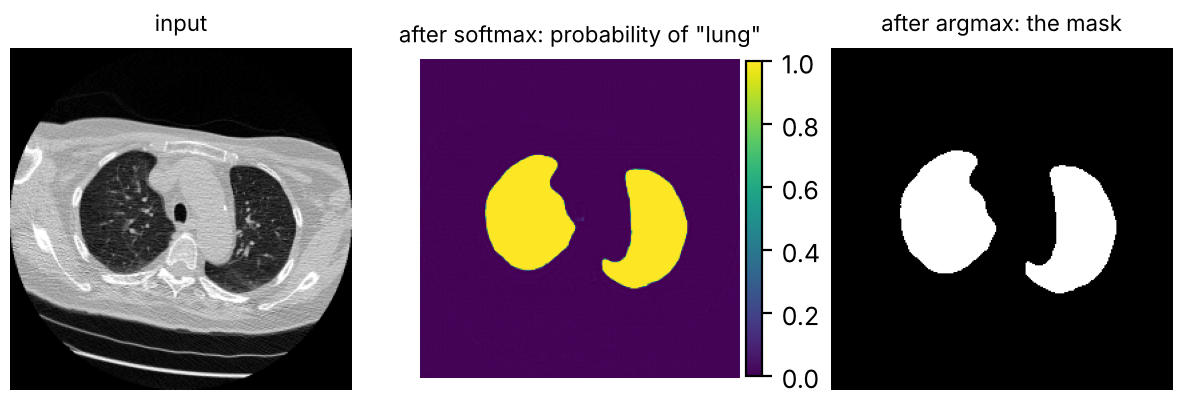
\includegraphics[width=0.95\linewidth]{output.png}
\end{center}

\remember{The U-Net goes down to understand what is in the image and up to say where; skip connections keep
the details. Its output is one score per class for each pixel; argmax gives the mask.}

% ---------------------------------------------------------------------------
\section{Loss and metric: the Dice}
\usedin{project STEP 7}

\subsection{The Dice score}

To compare a predicted mask $P$ with the true mask $T$ we measure how much they overlap:
\[
\text{Dice} = \frac{2\,|P \cap T|}{|P| + |T|}
\]
$|P \cap T|$ is the number of pixels that are lung in both masks; $|P|$ and $|T|$ are the lung pixels of each.

\begin{center}
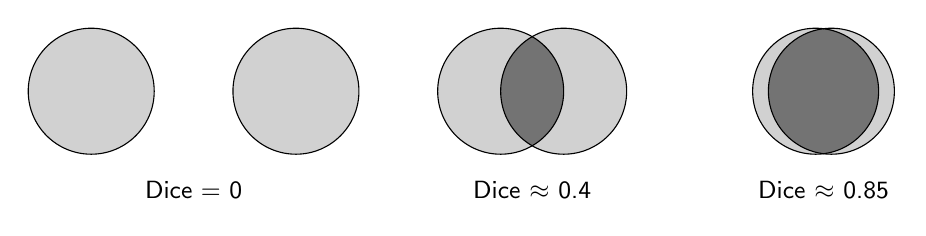
\begin{tikzpicture}[font=\small\sffamily]
\begin{scope}
  \fill[black!18] (0,0) circle (0.8); \fill[black!18] (2.6,0) circle (0.8);
  \draw (0,0) circle (0.8); \draw (2.6,0) circle (0.8);
  \node at (1.3,-1.25) {Dice = 0};
\end{scope}
\begin{scope}[xshift=5.2cm]
  \fill[black!18] (0,0) circle (0.8); \fill[black!18] (0.8,0) circle (0.8);
  \begin{scope} \clip (0,0) circle (0.8); \fill[black!55] (0.8,0) circle (0.8); \end{scope}
  \draw (0,0) circle (0.8); \draw (0.8,0) circle (0.8);
  \node at (0.4,-1.25) {Dice $\approx$ 0.4};
\end{scope}
\begin{scope}[xshift=9.2cm]
  \fill[black!18] (0,0) circle (0.8); \fill[black!18] (0.2,0) circle (0.8);
  \begin{scope} \clip (0,0) circle (0.8); \fill[black!55] (0.2,0) circle (0.8); \end{scope}
  \draw (0,0) circle (0.8); \draw (0.2,0) circle (0.8);
  \node at (0.1,-1.25) {Dice $\approx$ 0.85};
\end{scope}
\end{tikzpicture}
\end{center}

The Dice is 0 when the masks do not touch and 1 when they are identical.

\textbf{Why not accuracy?} Accuracy is the fraction of pixels classified correctly. Take a slice where the
lung is 10\% of the pixels, and a model that answers ``background'' everywhere:

\begin{center}
\begin{tabular}{@{}lcc@{}}
\toprule
 & Accuracy & Dice \\
\midrule
Model that predicts no lung at all & 90\% & 0 \\
\bottomrule
\end{tabular}
\end{center}

The model is useless and the accuracy says it is good. The Dice ignores the background, so it is not fooled
when the structure is small.

\subsection{Loss and metric are two different things}

\begin{itemize}
\item The \term{loss} is the number the training makes smaller. The network learns only from it.
\item The \term{metric} is the number we read to judge the model: the Dice score on the final masks, after
argmax.
\end{itemize}

Why not use the Dice score itself as the loss? Because of the argmax. To change the weights in the right
direction, the loss must change a little when the weights change a little (section 6.1). A mask does not: a
pixel is 0 or 1, and a small change of the weights usually leaves every pixel as it was. The Dice score would
stay identical and the network would get no information on how to improve.

\subsection{The Dice loss}

The \term{Dice loss} is the same formula computed on the \emph{probabilities} instead of the mask. For each
pixel $i$ let $p_i$ be the probability of ``lung'' given by the network (after softmax, between 0 and 1) and
$t_i$ the true label (0 or 1):
\[
\text{Dice loss} = 1 - \frac{2 \sum_i p_i\, t_i}{\sum_i p_i + \sum_i t_i}
\]
The sum $\sum_i p_i t_i$ is the ``soft'' overlap: it adds up the probability that the network gives to the
pixels that really are lung. The loss is 0 when the network gives probability 1 to every lung pixel and 0 to
all the others, and goes towards 1 as the overlap disappears. Every small change of a probability changes it,
so the network always knows in which direction to move.

An example on a row of six pixels:

\begin{center}
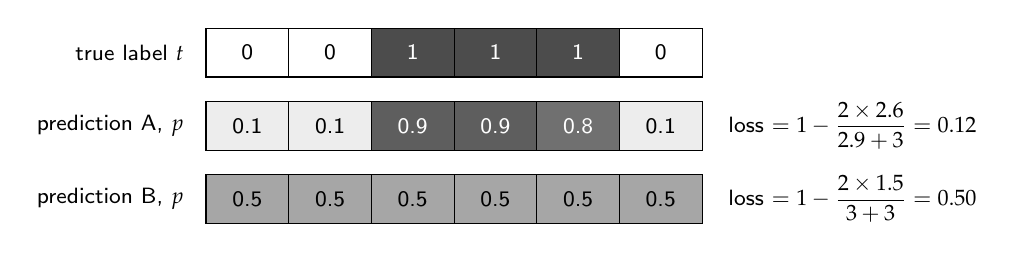
\begin{tikzpicture}[font=\footnotesize\sffamily, x=1.05cm, y=0.62cm]
% true labels
\node[anchor=east] at (-0.15,2.5) {true label $t$};
\foreach \i/\v/\g in {0/0/0, 1/0/0, 2/1/70, 3/1/70, 4/1/70, 5/0/0} {
  \draw[fill=black!\g] (\i,2) rectangle ++(1,1); \node[text=\ifnum\g>50 white\else black\fi] at (\i+0.5,2.5) {\v}; }
% prediction A
\node[anchor=east] at (-0.15,1.0) {prediction A, $p$};
\foreach \i/\v/\g in {0/0.1/7, 1/0.1/7, 2/0.9/63, 3/0.9/63, 4/0.8/56, 5/0.1/7} {
  \draw[fill=black!\g] (\i,0.5) rectangle ++(1,1); \node[text=\ifnum\g>50 white\else black\fi] at (\i+0.5,1.0) {\v}; }
\node[anchor=west] at (6.2,1.0) {loss $= 1 - \dfrac{2 \times 2.6}{2.9 + 3} = 0.12$};
% prediction B
\node[anchor=east] at (-0.15,-0.5) {prediction B, $p$};
\foreach \i in {0,...,5} { \draw[fill=black!35] (\i,-1) rectangle ++(1,1); \node at (\i+0.5,-0.5) {0.5}; }
\node[anchor=west] at (6.2,-0.5) {loss $= 1 - \dfrac{2 \times 1.5}{3 + 3} = 0.50$};
\end{tikzpicture}
\end{center}

Prediction A is right and fairly sure: low loss. Its mask after argmax is perfect (Dice score 1), yet the loss
is not 0: it still pushes the network to be more confident. Prediction B says ``I do not know'' everywhere:
high loss.

In the code:

\begin{center}
\code{loss\_function = DiceLoss(to\_onehot\_y=True, softmax=True)}
\end{center}

\begin{itemize}
\item \code{softmax=True}: the outputs of the network are scores; the loss turns them into probabilities itself.
\item \code{to\_onehot\_y=True}: our label is one image with 0 and 1; the loss rewrites it as two images, one
per class, to match the two output channels.
\item The loss is computed for each class and averaged.
\end{itemize}

\textbf{Cross-entropy}, the other common loss, looks at each pixel separately: it is small when the network
gives a high probability to the correct class of that pixel. It does not know about overlap, so with small
structures it is dominated by the background. \code{DiceCELoss} is the sum of the two (used in notebook 04).

\remember{Dice measures overlap, from 0 to 1, and is not fooled by a large background. The Dice loss is the
same formula on probabilities, so that it changes smoothly. The loss is for the training, the metric is for us.}

% ---------------------------------------------------------------------------
\section{Training}
\usedin{project STEP 8, 9, 10 and 11}

\subsection{The idea}

Training is a loop: show the network some images, measure how wrong it is, change the weights a little so that
it is less wrong, repeat.

How does it know in which direction to change millions of weights? For each weight PyTorch computes the
\term{gradient}: how much the loss would change if that weight changed a little. Moving every weight a small
step against its gradient makes the loss go down. This is \term{gradient descent}. The size of the step is the
\term{learning rate}. Too large: the loss jumps around and never settles. Too small: the training is very slow.

\begin{center}
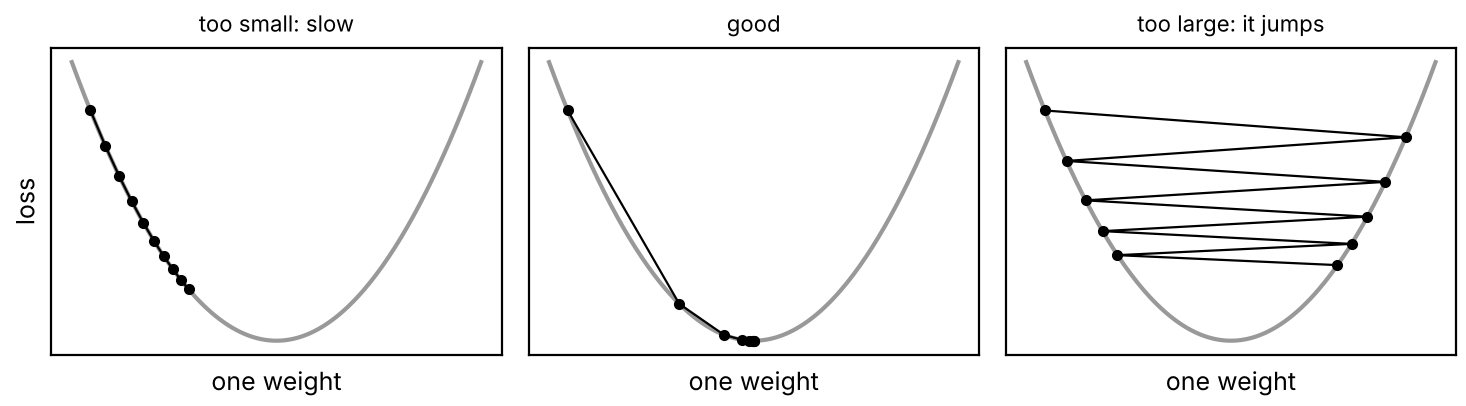
\includegraphics[width=0.9\linewidth]{learning_rate.png}

{\small Ten steps of gradient descent on a loss with one weight, with three learning rates.}
\end{center}

\subsection{One training step}

For each batch, five lines:

\begin{center}
\begin{tabular}{@{}cll@{}}
\toprule
 & Code & Meaning \\
\midrule
a & \code{optimizer.zero\_grad()} & delete the gradients of the previous step \\
b & \code{outputs = model(images)} & compute the predictions \\
c & \code{loss = loss\_function(outputs, labels)} & measure the error \\
d & \code{loss.backward()} & compute the gradients \\
e & \code{optimizer.step()} & change the weights \\
\bottomrule
\end{tabular}
\end{center}

The \term{optimizer} is the object that applies the change. We use Adam, a version of gradient descent that
adapts the size of the step for each weight.

\begin{center}
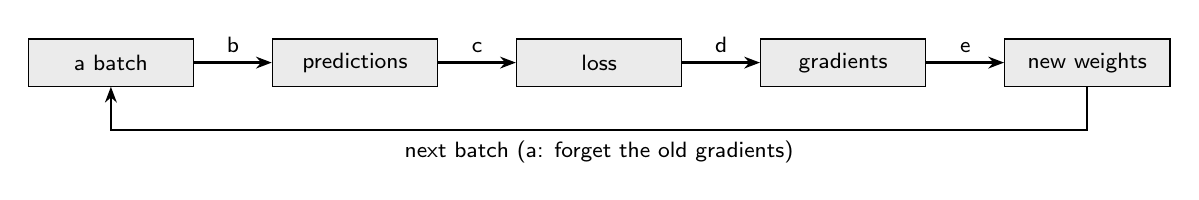
\begin{tikzpicture}[font=\footnotesize\sffamily,
  st/.style={draw, fill=black!8, minimum height=0.6cm, minimum width=2.1cm},
  arr/.style={-{Stealth[length=2mm]}, thick}]
\node[st] (b) at (0,0) {a batch};
\node[st] (f) at (3.1,0) {predictions};
\node[st] (l) at (6.2,0) {loss};
\node[st] (g) at (9.3,0) {gradients};
\node[st] (w) at (12.4,0) {new weights};
\draw[arr] (b) -- node[above] {b} (f);
\draw[arr] (f) -- node[above] {c} (l);
\draw[arr] (l) -- node[above] {d} (g);
\draw[arr] (g) -- node[above] {e} (w);
\draw[arr] (w.south) -- ++(0,-0.55) -| node[pos=0.25, below] {next batch (a: forget the old gradients)} (b.south);
\end{tikzpicture}
\end{center}

\subsection{Epochs and validation}

An \term{epoch} is one pass over all the training images. After each epoch we measure the Dice on the
validation set. Two details of the code:
\begin{itemize}
\item \code{model.train()} and \code{model.eval()} switch the network between training and evaluation mode
(some layers behave differently in the two);
\item \code{with torch.no\_grad():} tells PyTorch not to compute gradients, because during validation we do
not change the weights.
\end{itemize}

\subsection{Learning curves and overfitting}

\begin{center}
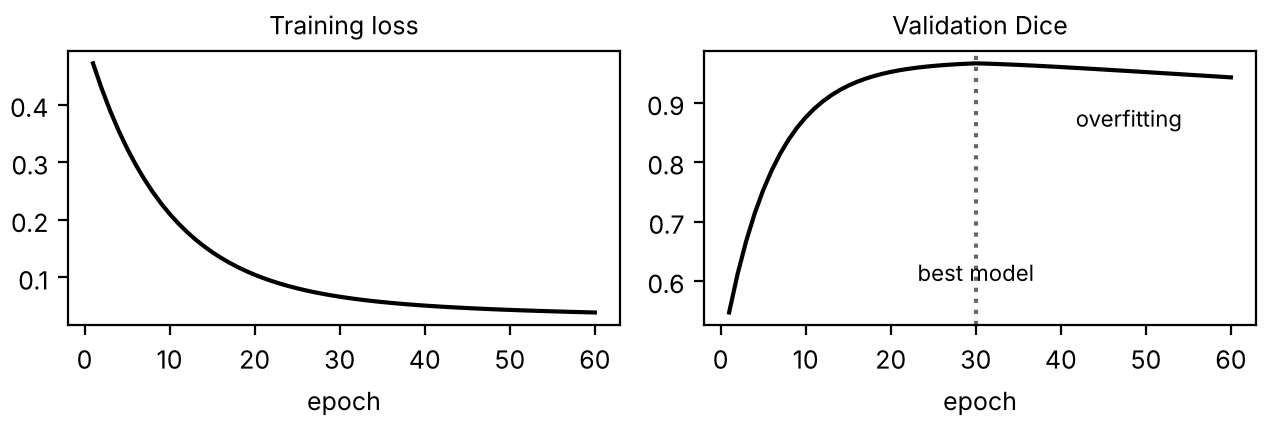
\includegraphics[width=0.85\linewidth]{curves.png}
\end{center}

The training loss goes down as long as we train. The validation Dice goes up, then flattens. If we continue,
the network starts to memorise the training images instead of learning what a lung looks like: the training
loss keeps improving while the validation Dice gets worse. This is \term{overfitting}.

This is why we save the weights every time the \emph{validation} Dice reaches a new maximum, and keep that
file as our model.

\subsection{If the training does not work}

\begin{center}
\begin{tabular}{@{}p{6.2cm}p{8.6cm}@{}}
\toprule
What you see & Likely cause \\
\midrule
The loss does not change & \code{loss.backward()} or \code{optimizer.step()} is missing \\
The loss jumps up and down & learning rate too large, or \code{zero\_grad()} is missing \\
The loss goes down, the Dice stays near 0 & labels are wrong: check the values of the mask after the
transforms \\
Error about devices & images or labels were not moved to the GPU with \code{.to(device)} \\
Error about sizes & print the shapes of images, labels and outputs \\
\bottomrule
\end{tabular}
\end{center}

\remember{Five lines per batch: zero\_grad, forward, loss, backward, step. Watch the validation Dice, not the
training loss, and keep the model with the best validation Dice.}

% ---------------------------------------------------------------------------
\section{Is the model good?}
\usedin{project STEP 12}

The test set gives the number to report. Three habits make that number honest.

\textbf{One value per patient, not only the mean.} A mean Dice of 0.97 can hide one patient at 0.60. Compute the
Dice of each patient, look at the distribution (minimum, histogram), and look at the worst cases.

\begin{center}
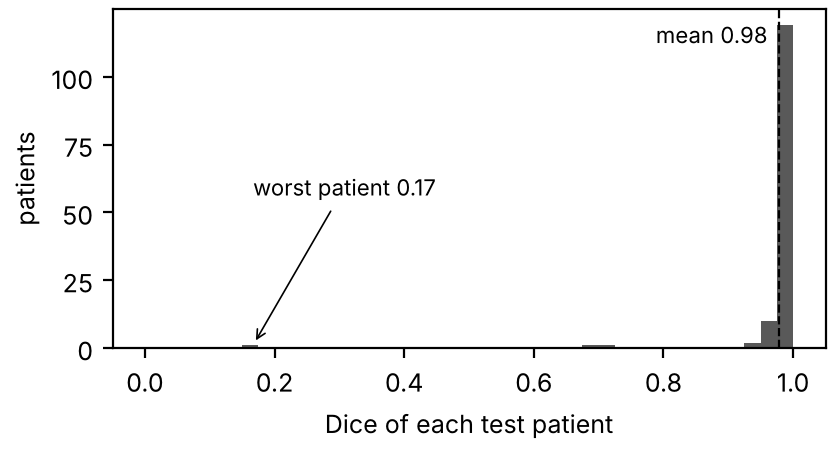
\includegraphics[width=0.55\linewidth]{test_dice.png}
\end{center}

\textbf{Look at the failures.} For each bad case ask: is the model wrong, or is the reference mask wrong? What
do the bad cases have in common (very small lungs at the top or bottom of the chest, disease, an unusual
scan)? The answers say where the model cannot be trusted.

\textbf{Know the limits of the data.} Our reference masks are automatic, so a high Dice means ``the model agrees
with another program''. All patients come from one public dataset of adults. A good result here is a good
student project, not a clinical tool.

\remember{Report the distribution, not only the mean. Look at the worst cases. Say what the data cannot tell.}

% ---------------------------------------------------------------------------
\section{Using the model}
\usedin{project STEP 13; web app}

\term{Inference} means using a trained model on a new image, with no mask and no training.

\textbf{What a saved model is.} The file \code{lung\_segmenter.pth} contains only the weights. To use it we must
first build the same network (same \code{channels}, same \code{strides}) and then load the weights into it.

\textbf{The rule of inference.} The model has learned from images prepared in one precise way: window
$-1000/400$ HU, rescaled to $0/1$, resized to $256 \times 256$. A new image must go through \emph{exactly the
same} preparation. If the application uses another window or another size, nothing crashes: the model simply
receives images unlike the ones it knows, and its predictions get worse silently. This is the most common
mistake when a model moves from a notebook to an application.

\begin{center}
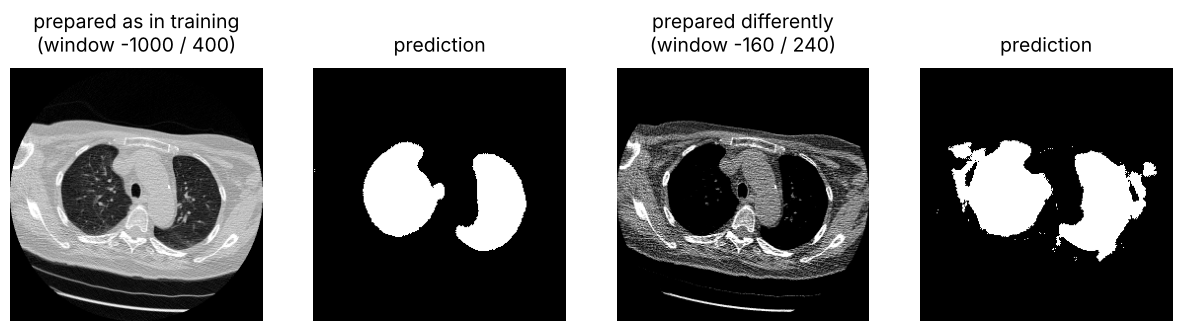
\includegraphics[width=0.98\linewidth]{skew.png}

{\small The same slice and the same model. On the right the image was rescaled with another window: no error
message, and a wrong mask.}
\end{center}

The steps of inference: load the file, prepare it as in the training, add the batch dimension, run the model
in evaluation mode without gradients, take the argmax.

\remember{A model is weights plus the exact preparation of its input. Change the preparation and the model
fails without telling you.}

% ---------------------------------------------------------------------------
\section{Lung nodules and experiments}
\usedin{notebook 04}

\subsection{Why nodules are harder than lungs}

A lung nodule is a small round lesion, from 3 to 30 mm. Segmenting it is a different problem from segmenting
the lung:

\begin{center}
\begin{tabular}{@{}lll@{}}
\toprule
 & Lung & Nodule \\
\midrule
Size in the image & a third of the slice & a few dozen pixels \\
Contrast & air against tissue & tissue against vessels and chest wall \\
Shape and position & always similar & anywhere, attached to anything \\
\bottomrule
\end{tabular}
\end{center}

Two consequences. First, \term{class imbalance}: almost every pixel is background, so a model that predicts
``no nodule'' everywhere is almost always right pixel by pixel.

\begin{center}
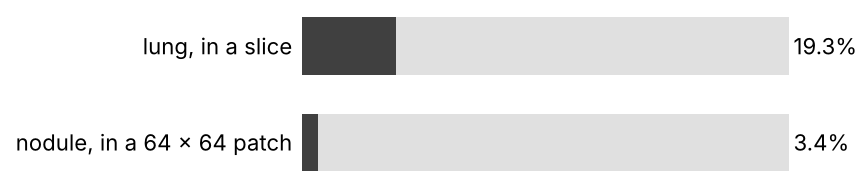
\includegraphics[width=0.7\linewidth]{imbalance.png}

{\small Share of the pixels that belong to the object, on average in our data.}
\end{center}

Second, with small objects the Dice is very sensitive. Suppose the model finds the object perfectly but draws
its border one pixel too wide all around:

\begin{center}
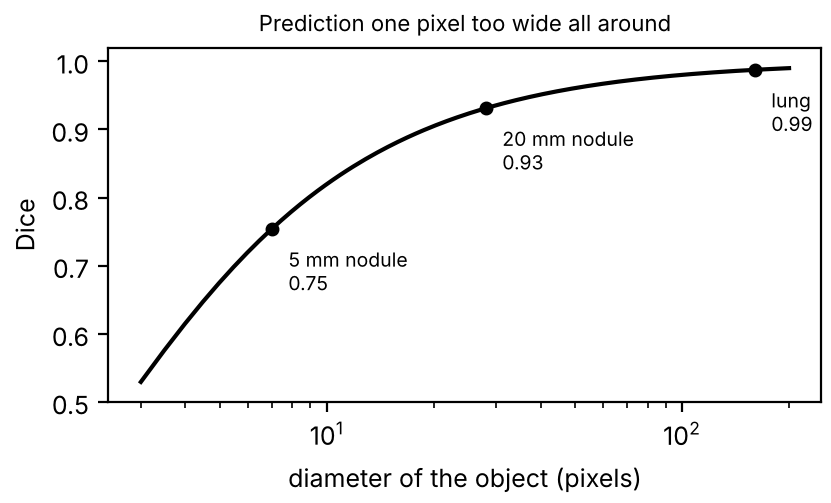
\includegraphics[width=0.6\linewidth]{dice_small.png}
\end{center}

The same one-pixel mistake costs nothing on a lung and a quarter of the score on a small nodule. Expect lower
and more variable scores.

To make the nodule visible to the network we do not give it the whole slice but a small \term{patch} cut
around the nodule.

\begin{center}
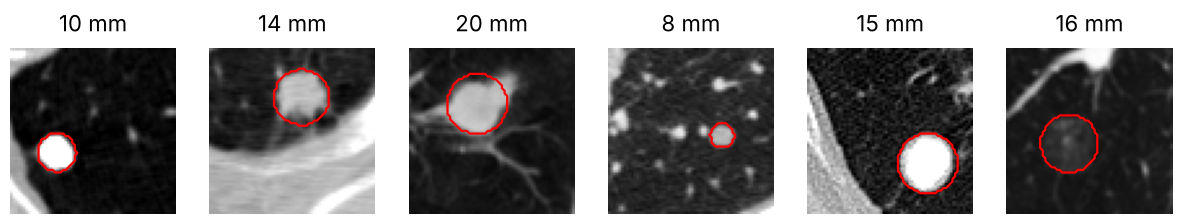
\includegraphics[width=0.95\linewidth]{nodules.png}

{\small Six patches of $64 \times 64$ pixels with the mask of the nodule (red) and its diameter.}
\end{center}

In our dataset the masks are discs: we know the centre and the diameter of each nodule, measured by
radiologists, but not its outline. Real nodules are not perfect circles, so no model can reach a Dice of 1
against these masks.

\subsection{How to run an experiment}

With lungs, almost any reasonable choice gives a Dice near 0.97. With nodules the choices matter, so this is
where we experiment. An experiment answers one question, and only if it is done in an orderly way:

\begin{enumerate}
\item \textbf{Start from a baseline.} Train a first model and write down its validation Dice.
\item \textbf{Change one thing.} If you change the loss and the learning rate together and the result
improves, you do not know which of the two helped.
\item \textbf{Write what you expect before you run.} One line. It forces you to think, and makes the
result informative even when it surprises you.
\item \textbf{Compare on the validation set}, with the same patients for every experiment.
\item \textbf{Do not trust small differences.} Train the same model twice with two different random seeds: the
two results differ. A change that improves the Dice by less than that difference has shown nothing.
\item \textbf{Keep a table}: what you changed, the result, what you conclude.
\end{enumerate}

The test set stays closed until you have chosen your final model.

\subsection{What can be changed}

\begin{center}
\begin{tabular}{@{}p{3.6cm}p{11.2cm}@{}}
\toprule
Choice & Idea \\
\midrule
Loss & The Dice loss alone can be unstable with tiny objects. Adding cross-entropy (\code{DiceCELoss}), which
judges every pixel, can make the training steadier. Whether it helps on our data is for you to measure. \\
Augmentation & For a round nodule, flips and rotations by any angle are realistic: more variety for free. \\
Learning rate & Ten times larger or smaller: look at how the curves change. \\
Size of the network & A smaller network may be enough for small patches, and overfits less. \\
Number of epochs & Small datasets overfit quickly: check where the validation Dice peaks. \\
Intensity window & A narrower window around lung and soft tissue gives the nodule more contrast. \\
\bottomrule
\end{tabular}
\end{center}

\remember{Small objects mean imbalance and unstable scores. Experiment one change at a time, against a
baseline, and compare differences with the noise between two identical runs.}

% ---------------------------------------------------------------------------
\section{From a model to a web app}
\usedin{day 5}

A model in a notebook is useful only to the person who wrote it. Turning it into something others can use
takes a few tools, each with one purpose.

\begin{center}
\begin{tabular}{@{}>{\raggedright}p{3.4cm}p{11.4cm}@{}}
\toprule
Tool & Purpose \\
\midrule
Virtual environment & A private copy of Python for one project, with its own packages. The file
\code{requirements.txt} lists them, so that anybody can rebuild the same environment. \\
Streamlit & Turns a Python file into a web page. The file is run from top to bottom at every action of the
user, so slow things, such as loading the model, are stored with \code{@st.cache\_resource}. \\
Git & Records the history of the files of a project: each \term{commit} is a saved version. \\
GitHub & Keeps a copy of the project online. The service that publishes the app reads the files from there. \\
Docker & Packs the app with everything it needs (operating system, Python, packages, model) into an
\term{image}. A running image is a \term{container}. The same image runs identically on any computer:
this is how software is installed in hospitals. \\
\bottomrule
\end{tabular}
\end{center}

\begin{center}
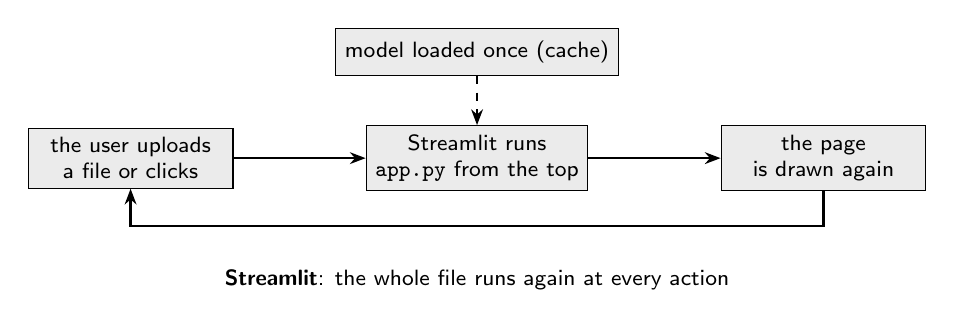
\begin{tikzpicture}[font=\footnotesize\sffamily,
  st/.style={draw, fill=black!8, minimum height=0.6cm, minimum width=2.6cm, align=center},
  arr/.style={-{Stealth[length=2mm]}, thick}]
\node[st] (u) at (0,0) {the user uploads\\a file or clicks};
\node[st] (r) at (4.4,0) {Streamlit runs\\\texttt{app.py} from the top};
\node[st] (p) at (8.8,0) {the page\\is drawn again};
\draw[arr] (u) -- (r); \draw[arr] (r) -- (p);
\draw[arr] (p.south) -- ++(0,-0.45) -| (u.south);
\node[st, minimum width=3.4cm] (c) at (4.4,1.35) {model loaded once (cache)};
\draw[arr, dashed] (c) -- (r);
\node at (4.4,-1.55) {\textbf{Streamlit}: the whole file runs again at every action};
\end{tikzpicture}
\end{center}

\begin{center}
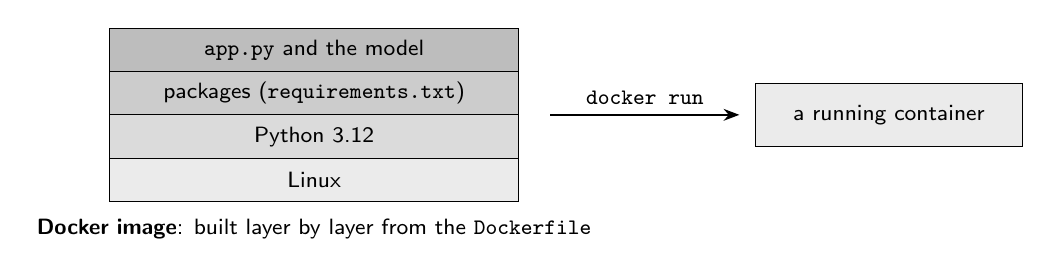
\begin{tikzpicture}[font=\footnotesize\sffamily]
\foreach \y/\t/\g in {0/Linux/8, 0.55/Python 3.12/14, 1.1/{packages (\texttt{requirements.txt})}/20, 1.65/{\texttt{app.py} and the model}/26} {
  \draw[fill=black!\g] (0,\y) rectangle ++(5.2,0.55); \node at (2.6,\y+0.275) {\t};
}

\draw[-{Stealth[length=2mm]}, thick] (5.6,1.1) -- node[above] {\texttt{docker run}} (8.0,1.1);
\draw[fill=black!8] (8.2,0.7) rectangle ++(3.4,0.8); \node at (9.9,1.1) {a running container};
\node at (2.6,-0.35) {\textbf{Docker image}: built layer by layer from the \texttt{Dockerfile}};
\end{tikzpicture}
\end{center}

\textbf{MLOps} is the name for everything that keeps a model working after the training: keeping track of
which data and which code produced which model, checking that the application prepares the data as in the
training, noticing when the model meets images unlike the ones it knows, and training it again when needed.

A public demo is not a medical device. Never upload real patient data to it.

% ---------------------------------------------------------------------------
\newpage
\section*{Index of terms}

\begin{center}
\begin{tabular}{@{}llp{9cm}@{}}
\toprule
Term & Section & In one line \\
\midrule
Argmax & 4.4 & the class with the highest score \\
Augmentation & 3.3 & random small changes of the training images \\
Batch & 3.1 & the images processed together \\
Channel & 3.1 & how many values each pixel has \\
Class imbalance & 9.1 & one class has far more pixels than the other \\
Container, image (Docker) & 10 & an app packed with everything it needs \\
Convolution & 4.2 & a small filter sliding over the image \\
DataLoader & 3.5 & groups the samples in batches \\
Dataset & 3.5 & gives sample number $i$ \\
Cross-entropy & 5.3 & a loss that judges each pixel separately \\
Dice & 5.1 & overlap between two masks, from 0 to 1 \\
Dice loss & 5.3 & the Dice formula on probabilities; what the training reduces \\
DICOM & 2 & clinical image format, one file per slice \\
Encoder, decoder & 4.3 & the two halves of the U-Net \\
Epoch & 6.3 & one pass over the training images \\
Gradient & 6.1 & how the loss changes when a weight changes \\
Ground truth & 1.4 & the mask taken as the correct answer \\
Hounsfield unit & 1.2 & the unit of CT values: water 0, air $-1000$ \\
Inference & 8 & using a trained model on new images \\
Interpolation & 3.2 & how new pixels are computed when resizing \\
Learning rate & 6.1 & the size of each change of the weights \\
Loss & 5.2 & the error that the training reduces \\
Mask, label & 1.4 & one whole number per pixel \\
Metric & 5.2 & the number we read to judge the model \\
NIfTI & 2 & research image format, one file per scan \\
Optimizer & 6.2 & the object that changes the weights \\
Overfitting & 6.4 & memorising the training images \\
Patch & 9.1 & a small piece cut from an image \\
Pixel spacing & 1.5 & the size of a pixel in millimetres \\
Skip connection & 4.3 & carries details from encoder to decoder \\
Softmax & 4.4 & turns scores into probabilities \\
Tensor, shape & 3.1 & the arrays of PyTorch and their dimensions \\
Training, validation, test & 3.4 & learn, check while learning, measure at the end \\
Transform & 3.2 & one step of the preparation of the data \\
U-Net & 4.3 & the standard network for segmentation \\
Virtual environment & 10 & a private Python for one project \\
Weights & 4.1 & the adjustable numbers of a network \\
Window & 1.3 & the range of HU that is shown or kept \\
\bottomrule
\end{tabular}
\end{center}

\end{document}
